\documentclass{article}
\usepackage[utf8]{inputenc}

\title{CS246 Homework 4 Answers}
\author{Charlie Zhang}
\date{Mar 2013}

\usepackage{tikz}
\usepackage{natbib}
\usepackage{float}
\usepackage{graphicx}
 \usepackage{indentfirst}
\usepackage{mathtools}
\usepackage{setspace}
\linespread{1.8}
\newenvironment{myenv}[1]
  {\begin{spacing}{#1}}
  {\end{spacing}}


\definecolor{sectionblue}{cmyk}{1,.75,0,0}
\definecolor{crimson}{cmyk}{.1,1,1,.1}
\usetikzlibrary{trees}
\tikzstyle{level 1} = [sibling distance=200pt]
\tikzstyle{level 2} = [sibling distance=100pt]
\tikzstyle{level 3} = [sibling distance=50pt]
\tikzstyle{innerNode} = [
 circle,
 draw=sectionblue!60,
 thick,
 top color=sectionblue!20,
 bottom color=sectionblue!40,
 align = center
]
\tikzstyle{leaf} = [
 rectangle,
 draw=crimson!70,
 thick,
 top color=crimson!15,
 bottom color=crimson!35,
 align = center,
 rounded corners,
 text width = 2em
]
  
\begin{document}

\maketitle
\section{Question 1 --Support Vector Machine}


\subsection{(a)}
The example:\\
(0, 0): -1 \\
(0, 1): -1 \\
(1, 0): 1 \\
(1, 1): 1 \\
(2, 0): -1 \\
This is unfeasible under hard constraints SVM but feasible under soft margin SVM. \\
Such as: $w = (2, 0), b = -1, \xi_1, .., \xi_5 = (0, 0, 0, 0, 4)$

\subsection{(b)}
Lets set: \\
$w_j = 0, \forall j = 1, ..., d, \\
 b = 0, \\
 \xi_i =  1, \forall i = 1, ..., n$ \\
 Then $y_i(w\cdot x + b) \ge 1 - \xi_i$ holds true for all i.

\subsection{(c)}
Let $T$ be the training set and $E$ be the set of points where linear classification mis-classified. \\
Then $y_i(x_i\cdot w + b) < 0, \forall i \in E$. \\
Also, $(w, \xi_i, ..., \xi_n)$ is a feasible point, so $y_i(x_i\cdot w + b) \ge 1 - \xi_i, \forall i \in T$
Now we have $1 - \xi_i < 0$, i.e., $\xi_i > 1$, $\forall i \in E$\\
So $\sum\limits_{i\in T}\xi_i >= \sum\limits_{i\in E}\xi_i > |E|$\\

\subsection{(d)}
$\nabla_b  f(w, b) = \frac{\delta f(w, b)}{\delta b} = C\sum\limits_{i=1}^{n}\frac{\delta L(x_i, y_i)}{\delta b}$ \\
Where $\frac{\delta L(x_i, y_i)}{\delta b} = \left\{ 
  \begin{array}{l l}
    0 & \quad \text{if $y_i(w\cdot x_i+b)\ge 1$}\\
    -y_i & \quad \text{otherwise}
  \end{array} \right. $

\subsection{(e)}
Red: BatchGradientDescend \\ Green: StochasticGradientDescend \\ Blue: MiniBatchGradientDescend\\
\begin{figure}[H]
\centering
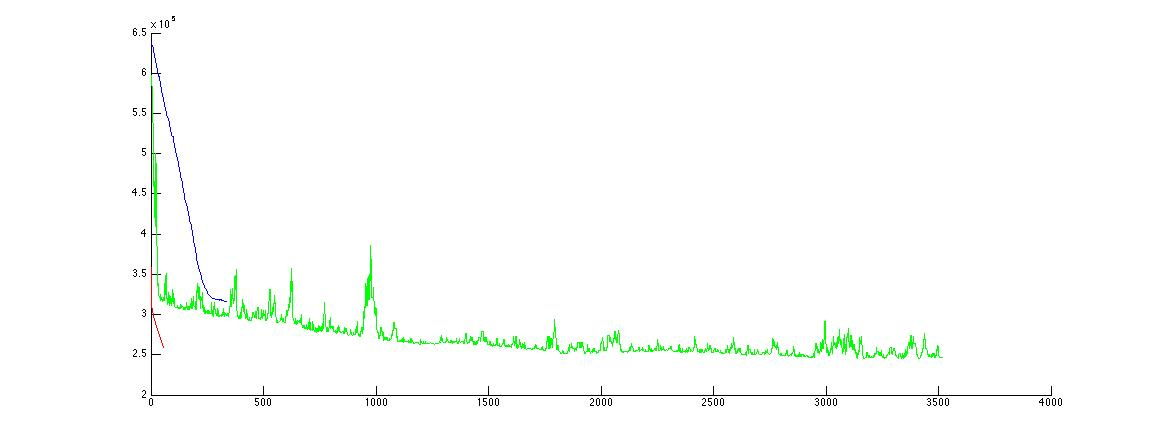
\includegraphics[scale=0.5]{q1e-cost.jpg}
\caption{ Cost as of iterations. }
\label{}
\end{figure}

\begin{figure}[H]
\centering
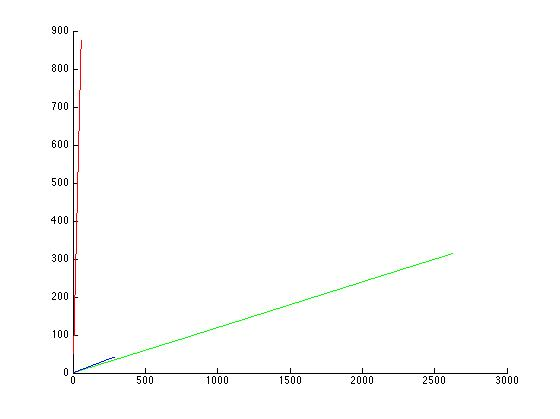
\includegraphics[scale=0.5]{q1e-time.jpg}
\caption{ Time elapsed as of iterations. }
\label{}
\end{figure}

What to infer: \\
Stochastic Gradient Descend makes many small but quick steps, some of the steps are wrong, but overall, it converges faster than Batch Gradient Descend in terms of computation time. But given sufficient computation resource, Batch Gradient Descend could achieve better result than Stochastic Gradient Descend.
Mini Batch Gradient Descend is a mixure of the two methods above, it makes more steps and runs faster than Batch Gradient Descend, the cost is also larger. It runs slower than Stochastic Gradient Descend, but it makes less error steps.

\subsection{(f)}
\begin{figure}[H]
\centering
\includegraphics[scale=0.5]{q1f.jpg}
\caption{ \textbf{\em{C}} Versus Percent Error. }
\label{}
\end{figure}

Conclusion: \\
Percent error gets smaller as \textbf{\em{C}} gets larger.

\section{Question 2 --Decision Tree Learning}
\subsection{(a)}
$G = max[I(D) - (I(D_L) + I(D_R))]$\\
There we only consider one attribute, so:\\
 $G = I(D) - (I(D_L) + I(D_R)) = \\ |D| \times (1-\sum\limits_ip_i^2) - |D_L| \times (1-\sum\limits_ip_{L(i)}^2) - |D_R| \times (1-\sum\limits_ip_{R(i)}^2) = \\
 |x + y + u + v| * ((1 - \frac{(x+u)^2}{(x+y+u+v)^2}) + (1 - \frac{(y+v)^2}{(x+y+u+v)^2})) -
 |x + y| * ((1 - \frac{x^2}{x+y)^2}) + (1 - \frac{y^2}{x+y)^2})) -
 |u + v| * ((1 - \frac{u^2}{u+v)^2}) + (1 - \frac{v^2}{u+v)^2})) = \\
 \frac{x^2+y^2}{x+y}+ \frac{u^2+v^2}{u+v} - \frac{(x+u)^2+(y+v)^2}{x+y+u+v} > 0$\\
 Solve the inequality and we get $(xv - yu)^2 > 0$. \\
 So $\frac{x}{y} \ne \frac{u}{v}$.
 
 
 \subsection{(b)}
 based on the equation in (a), we have: \\
 $G_{wine} = \frac{30^2+20^2}{50}+ \frac{30^2+20^2}{50} - \frac{60^2+40^2}{100} = 0$ \\
 $G_{running} = \frac{20^2+10^2}{30}+ \frac{40^2+30^2}{70} - \frac{60^2+40^2}{100} = 0.381$ \\
 $G_{pizza} = \frac{50^2+30^2}{80}+ \frac{10^2+10^2}{20} - \frac{60^2+40^2}{100} = 0.500$ \\
 We should use the attribute 'likes pizza'

 \subsection{(c)}
The decision tree is a complete binary tree with a depth of 100. \\
There are $2^{100}$ leaf nodes, which are the decision nodes, corresponding to the $\{0,1\}^{100}$ feature space. \\
The root is $a_1$, the two branches are $a_1=0$ and $a_1=1$ respectively, the rest of the tree (2nd layer to leaf) are nodes for $a_2 ... a_{100}$, the arrangement of $a_2 ... a_{100}$ in these nodes are arbitrary, depending on the features of those elements whose target value not equal to $a_1$. \\

A desired decision tree should have a depth of 1, and 2 leaf nodes. \\
The decision criterion are $a_1 = 0$ and $a_1 = 1$. \\
This tree will not over fit to those 1\% training data whose target value not equals to $a_1$.
 \subsection{(d)}
$T_0:$

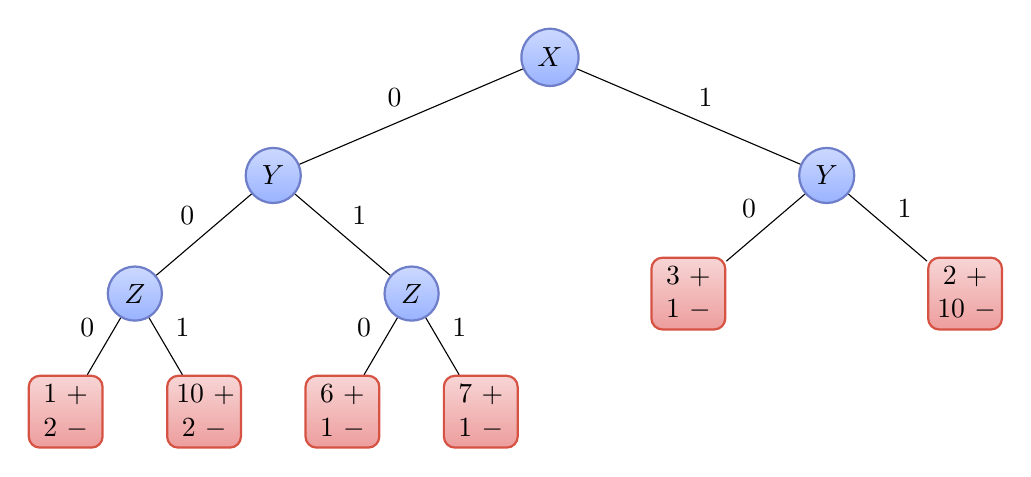
\begin{tikzpicture}
  \node [innerNode] (z) {$X$}
    child {
      node [innerNode] (a) {$Y$}
      child {
        node [innerNode] (b) {$Z$}
        child {
          node [leaf] (k) {$1\ +$ \\ $2\ -$}
          edge from parent node[above left] {$0$}
        }
        child {
          node [leaf] (k) {$10\ +$ \\ $2\ -$}
          edge from parent node[above right] {$1$}
        }
        edge from parent node[above left] {$0$}
      }
      child {
        node [innerNode] (g) {$Z$}
        child {
          node [leaf] (k) {$6\ +$ \\ $1\ -$}
          edge from parent node[above left] {$0$}
        }
        child {
          node [leaf] (k) {$7\ +$ \\ $1\ -$}
          edge from parent node[above right] {$1$}
        }
        edge from parent node[above right] {$1$}
      }
      edge from parent node[above left] {$0$}
    }
    child {
      node [innerNode] (a) {$Y$}
      child {
        node [leaf] (b) {$3\ +$ \\ $1\ -$}
        edge from parent node[above left] {$0$}
    }
    child {
      node [leaf] (g) {$2\ +$ \\ $10\ -$}
      edge from parent node[above right] {$1$}
    }
    edge from parent node[above right] {$1$}
  };
\end{tikzpicture}
\\

$T_1$:

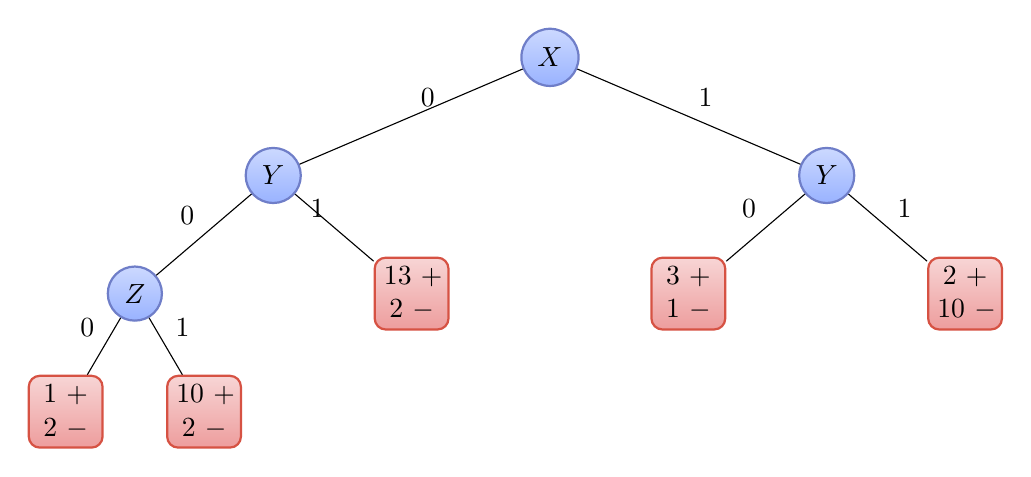
\begin{tikzpicture}
  \node [innerNode] (z) {$X$}
    child {
      node [innerNode] (a) {$Y$}
      child {
        node [innerNode] (b) {$Z$}
        child {
          node [leaf] (k) {$1\ +$ \\ $2\ -$}
          edge from parent node[above left] {$0$}
        }
        child {
          node [leaf] (k) {$10\ +$ \\ $2\ -$}
          edge from parent node[above right] {$1$}
        }
        edge from parent node[above left] {$0$}
      }
      child {
          node [leaf] (k) {$13\ +$ \\ $2\ -$}
          edge from parent node[above left] {$1$}
       }
       edge from parent node[above right] {$0$}
    }
    child {
      node [innerNode] (a) {$Y$}
      child {
        node [leaf] (b) {$3\ +$ \\ $1\ -$}
        edge from parent node[above left] {$0$}
    }
    child {
      node [leaf] (g) {$2\ +$ \\ $10\ -$}
      edge from parent node[above right] {$1$}
    }
    edge from parent node[above right] {$1$}
  };
\end{tikzpicture}

$T_2$:

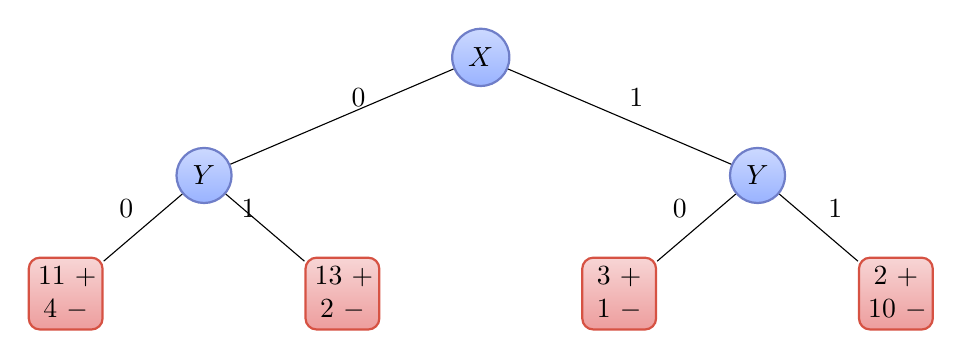
\begin{tikzpicture}
  \node [innerNode] (z) {$X$}
    child {
      node [innerNode] (a) {$Y$}
      child {
        node [leaf] (k) {$11\ +$ \\ $4\ -$}
        edge from parent node[above left] {$0$}
      }
      child {
          node [leaf] (k) {$13\ +$ \\ $2\ -$}
          edge from parent node[above left] {$1$}
       }
       edge from parent node[above right] {$0$}
    }
    child {
      node [innerNode] (a) {$Y$}
      child {
        node [leaf] (b) {$3\ +$ \\ $1\ -$}
        edge from parent node[above left] {$0$}
    }
    child {
      node [leaf] (g) {$2\ +$ \\ $10\ -$}
      edge from parent node[above right] {$1$}
    }
    edge from parent node[above right] {$1$}
  };
\end{tikzpicture}

$T_3$:

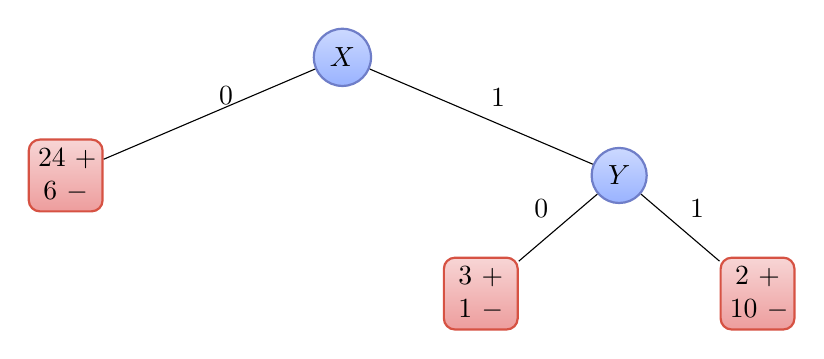
\begin{tikzpicture}
  \node [innerNode] (z) {$X$}
    child {
      node [leaf] (k) {$24\ +$ \\ $6\ -$}
      edge from parent node[above right] {$0$}
    }
    child {
      node [innerNode] (a) {$Y$}
      child {
        node [leaf] (b) {$3\ +$ \\ $1\ -$}
        edge from parent node[above left] {$0$}
    }
    child {
      node [leaf] (g) {$2\ +$ \\ $10\ -$}
      edge from parent node[above right] {$1$}
    }
    edge from parent node[above right] {$1$}
  };
\end{tikzpicture}

$T_4$, obtained with $\alpha=\frac{2}{45}$:

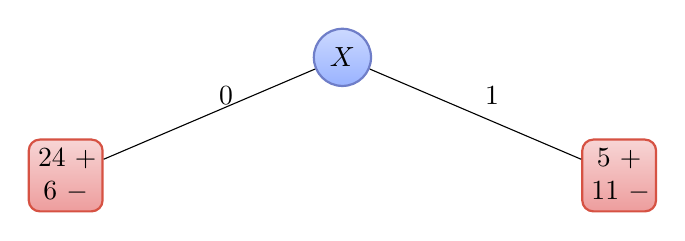
\begin{tikzpicture}
  \node [innerNode] (z) {$X$}
    child {
      node [leaf] (k) {$24\ +$ \\ $6\ -$}
      edge from parent node[above right] {$0$}
    }
    child {
      node [leaf] (g) {$5\ +$ \\ $11\ -$}
      edge from parent node[above right] {$1$}
  };
\end{tikzpicture}

$T_5$:

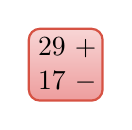
\begin{tikzpicture}
    \node [leaf] (k) {$29\ +$ \\ $17\ -$};
\end{tikzpicture}

\subsection{(e)}
Generalization errors for \{$T_0$ ... $T_5$\} are: \\
\{$\frac{2}{4}$, $\frac{2}{4}$, $\frac{1}{4}$, $\frac{1}{4}$, $0$, $\frac{2}{4}$\}. \\
$T_4$ is the one with best generalization error.


\section{Question 3 --Clustering Data Streams}
\subsection{(a)}
$2a^2 + 2b^2 - (a+b)^2 = \\
2a^2 + 2b^2 - (a^2 + 2ab + b^2) =\\
a^2 - 2ab + b^2 =\
(a-b)^2 \ge 0$.\\
So $(a+b)^2 \le 2a^2 + 2b^2$.

\subsection{(b)}
Based on conclusion in (a), we have $2d(x, y)^2 + 2d(y, T)^2 \ge (d(x,y)+d(y,T))^2 \ge d(x, T)^2$, $\forall x,y \in S, \forall T$.  \\
$2\cdot cost_w(\hat S,T) + 2\sum\limits_{i=1}^{l}cost(S_i, T_i) = \\
2 \sum\limits_{i=1}^{l}\sum\limits_{j=1}^{k}|S_{ij}|d(t_{ij}, T)^2 + 2\sum\limits_{i=1}^{l}\sum\limits_{j=1}^{k}\sum\limits_{x \in S_{ij}} d(x,t_{ij})^2 = \\
\sum\limits_{i=1}^{l}\sum\limits_{j=1}^{k}\sum\limits_{x \in S_{ij}} (2d(x,t_{ij})^2 + 2d(t_{ij},T)^2) \ge \\
\sum\limits_{i=1}^{l}\sum\limits_{j=1}^{k}\sum\limits_{x \in S_{ij}}d(x,T)^2 =\\
cost(S,T)$

\subsection{(c)}
$\sum\limits_{i=1}^{l}cost(S_i,T_i) \le \alpha\sum\limits_{i=1}^{l}cost(S_i, T_i^*)$, where $T_i^*$ is the optimal solution for $S_i$ \\
Since $T_i^*$ is the optimal solution for $S_i$, $cost(S_i, T_i^*) \le cost(S_i, T^*)$.\\
$\sum\limits_{i=1}^{l}cost(S_i, T_i^*) \le \sum\limits_{i=1}^{l}cost(S_i, T^*) = cost(S, T^*)$ \\
So $\sum\limits_{i=1}^{l}cost(S_i,T_i) \le \alpha \cdot cost(S, T^*)$.

\subsection{(d)}
According to the definition of ALG, $cost_w(S,T) \le \alpha \min\limits_{|T^\prime|=k}\{cost_w(S,T^\prime)\}$.
$T$ is obtained by running ALG on $\hat S$, by definition, we have:\\
$cost_w(\hat S,T) \le \alpha cost_w(\hat S,T^*)$

\subsection{(e)}
$2\sum\limits_{i=1}^lcost(S_i, T_i) + 2cost(S,T^*) =\
2\sum\limits_{i=1}^{l}\sum\limits_{j=1}^{k}\sum\limits_{x \in S_{ij}} d(x,t_{ij})^2 + 2\sum\limits_{x \in S}d(x,T^*)^2 = \\
\sum\limits_{i=1}^{l}\sum\limits_{j=1}^{k}\sum\limits_{x \in S_{ij}} 2(d(x, t_{ij})^2 + d(x,T^*)^2) \ge \\
\sum\limits_{i=1}^{l}\sum\limits_{j=1}^{k}\sum\limits_{x \in S_{ij}} (d(x, t_{ij}) + d(x, T^*))^2 \ge \\
\sum\limits_{i=1}^{l}\sum\limits_{j=1}^{k}|S_{ij}|d(t_{ij}, T^*)^2) =\\
cost_w(\hat S, T^*)$ \\
So, $cost_w(\hat S, T^*) \le 2\sum\limits_{i=1}^lcost(S_i, T_i) + 2cost(S,T^*)$

\subsection{(f)}
Based on conclusions in (b), (c), (d), (e), we have: \\
$cost(S,T) \le 2\cdot cost_w(\hat S,T) + 2\sum\limits_{i=1}^{l}cost(S_i, T_i) =\\ 
2\alpha \cdot cost_w(\hat S, T^*) + 2\alpha \cdot cost(S,T^*) \le\\
2\alpha \cdot (2\sum\limits_{i=1}^lcost(S_i, T_i) + 2cost(S,T^*) )  + 2\alpha \cdot cost(S,T^*) \le \\
2\alpha \cdot (2\alpha \cdot cost(S,T^*) + 2cost(S,T^*) )  + 2\alpha \cdot cost(S,T^*) = \\
(4\alpha^2 + 6\alpha)\cdot cost(S,T^*)$

\subsection{(g)}
Assumes that we know the value of $n$ in the first place. \\
Set number of partition $l = \sqrt{\frac{n}{k}}$, then, $|S_i| = \frac{|S|}{l} = \sqrt{nk}, \forall i=1,...,l$. \\
Maximum space requirement = \\ Space for storing $S_i$ and run ALG on $S_i$ plus space for storing $T$, and space for running ALG on $T$ =\\
 max( (space of ALG for $S_i$) $+ kl$, space of ALG for $\hat S$) \\
= max($\frac{n}{l}$ + kl, kl) \\
= $\sqrt{nk}$

With choices of $l = \sqrt{\frac{n}{k}}$, assuming that we know $n$ ahead, \\
ALGSTR works with O($\sqrt{nk}$) space.

\section{Question 4 -- Data Streams}
\subsection{(a)}
Every occurrence of $i$, we increment the count $c_{j,h_j(i)}$, $\forall j \in [[1; [log\frac{1}{\delta}]]]$. \\
Suppose there are no other elements than $i$ in the stream, then $c_{j,h_j(i)} = F[i]$, $\forall j \in [[1; [log\frac{1}{\delta}]]]$ \\ 
In this case $min_j\{c_{j,h_j(i)}\} = F[i]$ \\
Since there could be other elements in the stream that collides with $i$ in hashed values, so overall, $\tilde F[i] = min_j\{c_{j,h_j(i)}\} \ge F[i]$

\subsection{(b)}
Since $h_j$ maps \{1,2,...n\} to $\{1,2,...[\frac{e}{\epsilon}]\}$ uniformly, the expected number of other elements falls in $c_{j,h_j(i)}$ for hash function $j$ is: \\
$\frac{(t-F[i])}{[\frac{e}{\epsilon}]}$. \\
So, for any $1 \le i \le n$ and $1 \le j \le [log\frac{1}{\delta}]$ ,  $E[c_{j, h_j}] = F[i] + \frac{(t-F[i])}{[\frac{e}{\epsilon}]} \le F[i]+\frac{\epsilon}{e}(t-F[i])$.

\subsection{(c)}
$Pr[\tilde F[i]\le F[i]+\epsilon t] = 1-(Pr[c_{j,h_j(i)} > F[i] + \epsilon t])^{[log\frac{1}{\delta}]}$ \\
Based on Markov's Inequality, \\ $Pr[c_{j,h_j(i)} > F[i] + \epsilon t]  =  \\
Pr[c_{j,h_j(i)} - F[i] > \epsilon t]  \le \\
 \frac{E[c_{j,h_j(i)} - F[i]]}{\epsilon t} \le \\
  \frac{F[i]+\frac{\epsilon}{e}(t-F[i]) - F[i]}{\epsilon t} \le   \frac{\frac{\epsilon}{e}t}{\epsilon t} = \frac{1}{e}$
So $Pr[\tilde F[i]\le F[i]+\epsilon t] =  \\
1-(Pr[c_{j,h_j(i)} > F[i] + \epsilon t])^{[log\frac{1}{\delta}]} \ge
1 - \frac{1}{e}^{log\frac{1}{\delta}} = 1 - \delta$ \\

\subsection{(d)}
In HW3-Q4, we need $O(n)$ extra memory to keep track of the degree of each node, where $n$ is the number of nodes.\\
With the approach provided above, we can bring down the extra memory requirement from $O(n)$ to $O(\frac{1}{\epsilon}log[\frac{1}{\delta}])$.

\begin{myenv}{0.8}
\begin{verbatim}
\end{verbatim}
\end{myenv}

\end{document}